\documentclass[a4paper, parskip=true, firsthead=false, fromemail=true, foldmarks=false]{scrlttr2}
\usepackage[utf8]{inputenc}
\setkomavar{fromemail}{thomas.gibaud@ens-lyon.fr}
\setkomavar{signature}{Mathieu Leocmach,\\ Mathieu Nespoulous,\\ Sébastien Manneville,\\ Thomas Gibaud\\
{\small Ecole Normale Supérieure de Lyon}}


\usepackage{amsmath}
\usepackage{amsfonts}
\usepackage{amssymb}
\usepackage{graphicx}
\usepackage[british]{babel}

\usepackage{kpfonts}
\usepackage{tabu}

\begin{document}
\begin{letter}{From:\\
Thomas Gibaud,\\
Laboratoire de physique,\\
Ecole Normale Supérieure de Lyon,\\
\texttt{thomas.gibaud@ens-lyon.fr}
}
\opening{\bf Dear Editor,}

Please find enclosed our manuscript, entitled \emph{Hierarchical wrinkling in permeable and confined biogels}, which we are submitting for publication as an article to Nature Materials.



Supplementary video 1 arouse one's curiosity. It shows microscopy images of the biogel as a function of time in and optical cell where the adhesion of the protein to the cell wall is prohibited. How can a simple protein gel form spontaneously such complicated nested patterns?

Supplementary video 2, which shows a 3D construction of the gel based on confocal imaging, hints towards the answer. The gel shrinks then swells and wrinkles due to the excess area created during swelling. This is however not the end of the story as boundary conditions frustrate the development of the wrinkles and induce buckling within the buckling . This hierarchical pattern is a beautiful illustration of the well known Droste effect named after the cacao brand whoes trademark image displays a nurse carrying a serving tray with a cup of hot chocolate and a box with the same image. In France it is known as the    ``Vache qui rit'' effect and of course one thinks about Russian dolls.


\begin{tabu}{X[c]X[c]}
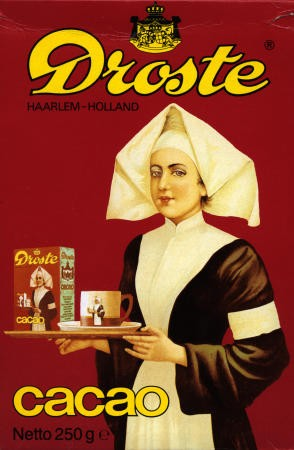
\includegraphics[height=6\baselineskip]{../Droste.jpg}&
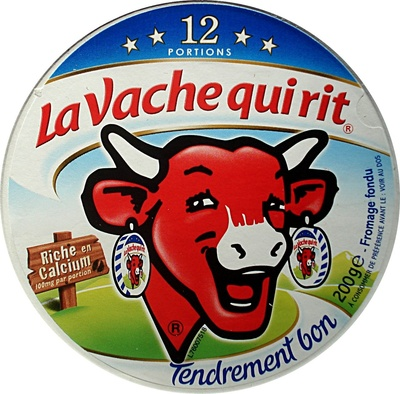
\includegraphics[height=6\baselineskip]{../vachequirit.jpg}
\end{tabu}



It is universally recognized that confined thin surfaces may wrinkle due the growth of an excess of material. For example on the biology side different rates of growth between the gut tube and its dorsal anchoring is responsible for the vilification of guts. Localized cell death in biofilms focuses mechanical forces and initiates 3D labyrinth pattern. Such patterns can also be triggered by physical cues as temperature dilation, swelling or the removal of pre-strain.

Yet, benchmark experiments such as the one presented in Supplementary Video 1 and 2, that explore the possibility of wrinkling in confined porous soft materials immersed in a buoyancy-matched viscous medium are in line. Indeed, stability analysis of a film lying on a thin viscous substrate was studied only recently and remains theoretical because, on a free interface, gravity dominates over viscous substrate.

From a fundamental perspective, our work unifies concepts from diverse soft matter systems.
\begin{enumerate}
\item From food science we have hijacked the process of yoghurt making to form gels. Usually, when you acidify milk the caseins flocculate. To form a uniform yoghurt gel one needs to lower homogeneously the pH, as bacteria do. Here we use the acidulent GDL for finer control.

\item  Next, we exploit the concept of stability in colloidal suspensions. As the GDL acidifies the medium, caseins loose their net charge and aggregate. Upon further acidification the casein regain charges and partially desorb form the gel. This makes the gel successively shrink and swell.

\item This process also can be well understood by invoking two different theories of gelation. Diffusion limited cluster aggregation is responsible for the formation of the fractal network of the gel ; whereas arrested phase separation well describes the coexistence between a dilute phase and a dense glassy network.

\item Finally, we invoke hydrodynamics with the seminal work of Darcy and Poiseuille. In particular we demonstrate the kinetic selection of the wavelength due to two sources of viscous dissipation. We predict the wrinkling wavelength invoking Poiseuille flows of the solvent above and below the gel layer for long wavelengths and a new mechanism, Darcy flows of the solvent through the gel layer for short wavelengths.
\end{enumerate}



From a practical perspective, such a model experiment, because it relies on pH induced charge stabilisation/destabilisation, should be generalisable to different sort of proteins. Controlled gelation with peculiar boundary conditions introduces a robust method to produce wrinkled surfaces that is distinct from other emerging technologies. We use a combination of complementary techniques ranging from polymer brush grafting, titration, light microscopy, rheology, permeability measurements and confocal microscopy that sustains studies to better understand the relations between all levels of hierarchy from the individual proteins to the macroscopic. Indeed, we directly measure and relate the non monotonous pH response of the proteins to the spontaneous shrinkage and swelling effect of the casein network at the micron level to the wrinkles at the millimetre scale. Playing with the geometry, the gel composition and the viscosity of the solvent, we explore a wide range of physical parameters to check the validity of our models. All of these differences enable us to assemble, to our knowledge, the first example of Darcy flow driven wrinkling.

The impact of our work extends beyond soft-matter physics. For instance, it illustrates daily life problems such as wrinkles encountered while putting up wall paper and could set a benchmark to explore potential applications in micro-fingerprinting or in optical devices such as diffraction gratings or Fresnel lenses, and the possibility of wrinkling in confined porous soft materials immersed in a buoyancy-matched viscous medium such as biological tissues. Indeed during the morphogenesis of the embryo the development of confined permeable and wrinkled surface is ubiquitous.


For all these reasons we believe that our manuscript is suitable for a publication in an interdisciplinary journal such as XXX. With this manuscript we are including XXX supplementary movies, which have been mailed to your editorial office. As possible reviewers we suggest: L. Mahadevan (Harvard, USA), N. Menon (Amherst, USA), José Bico (ESPCI, France), Enrique Cerda (Univ. Santiago-Chile, Chile), Mokhtar-Adda-Bedia (ENS Paris, France), Shu Yang (U.Penn, USA), Pascal Damman (Univ. Mons, Belgium), Tian Yang (Univ. Michigan, USA), Dominic Vella (Oxford, UK) XXX.

 

We thank you for your time and attention.

\closing{\bf Sincerely yours,} 

\end{letter} 
\end{document}